% Figure s09f01_nesting (Session 9): nesting is what makes a response function diverge.
% The image is rendered by figures/blender/s09f01_nesting.py; the coordinates of the labels come from
% figures/blender/out/s09f01_nesting*_anchors.tex. Build with figures/blender/build_figure.sh s09f01_nesting.
\documentclass[11pt,tikz,border=0pt]{standalone}
\usepackage[T1]{fontenc}
\usepackage{amsmath,amssymb,graphicx,bm}
\usepackage{xcolor}
\usetikzlibrary{arrows.meta,calc}
% The three label colors of the figures, with the same values as in src/figures_preamble.tex.
\definecolor{aqmaccent}{RGB}{31,78,121}
\definecolor{aqmbroken}{RGB}{168,42,34}
\definecolor{aqmmuted}{RGB}{125,125,125}

% Shared TikZ styles of the overlays: axis arrows drawn on top of the renders, between anchors
% written by the scripts, so that they can be adjusted without rendering again.
\tikzset{
  axarrow/.style={line width=0.6pt, draw=black!70, -{Stealth[length=4.5pt,width=3.5pt]}},
  axlbl/.style={font=\small, inner sep=1.5pt},
}
% A discrete color key: \aqmkey{(x,y)}{color 1}{label 1}{color 2}{label 2} draws two swatches in a
% column with their labels, anchored at its north west corner. The colors are the sRGB values
% used in the render, defined below.
\definecolor{keypos}{RGB}{118,158,198}
\definecolor{keyneg}{RGB}{214,150,132}
\definecolor{keyup}{RGB}{224,62,40}
\definecolor{keydown}{RGB}{40,92,200}
\definecolor{keydark}{RGB}{31,78,121}
\definecolor{keylight}{RGB}{118,158,198}
\newcommand{\aqmkey}[5]{%
  \begin{scope}[shift={#1}]
    \fill[#2, draw=black!40, line width=0.3pt] (0,-0.32) rectangle (0.32,0);
    \node[font=\small, anchor=west, inner sep=1.5pt] at (0.38,-0.16) {#3};
    \fill[#4, draw=black!40, line width=0.3pt] (0,-0.74) rectangle (0.32,-0.42);
    \node[font=\small, anchor=west, inner sep=1.5pt] at (0.38,-0.58) {#5};
  \end{scope}}
% The same key in one row, for a figure with no room for a column.
\newcommand{\aqmkeyrow}[5]{%
  \begin{scope}[shift={#1}]
    \fill[#2, draw=black!40, line width=0.3pt] (0,-0.32) rectangle (0.32,0);
    \node[font=\small, anchor=west, inner sep=1.5pt] (k1) at (0.38,-0.16) {#3};
    \fill[#4, draw=black!40, line width=0.3pt] ([xshift=0.25cm]k1.east |- 0,-0.32) rectangle ++(0.32,0.32);
    \node[font=\small, anchor=west, inner sep=1.5pt] at ([xshift=0.63cm]k1.east) {#5};
  \end{scope}}

\newlength{\figw}\setlength{\figw}{15.60cm}   % the text width of the notes (A4, 2.7 cm margins)

\begin{document}
\begin{tikzpicture}[lbl/.style={font=\small, inner sep=1.5pt}, pnl/.style={font=\small\bfseries, inner sep=1.5pt}]
  \begin{scope}[shift={(0.00cm,0.00cm)}]
    \setlength{\figw}{10.40cm}
    \node[overlay, anchor=south west, inner sep=0pt] at (0,0)
      {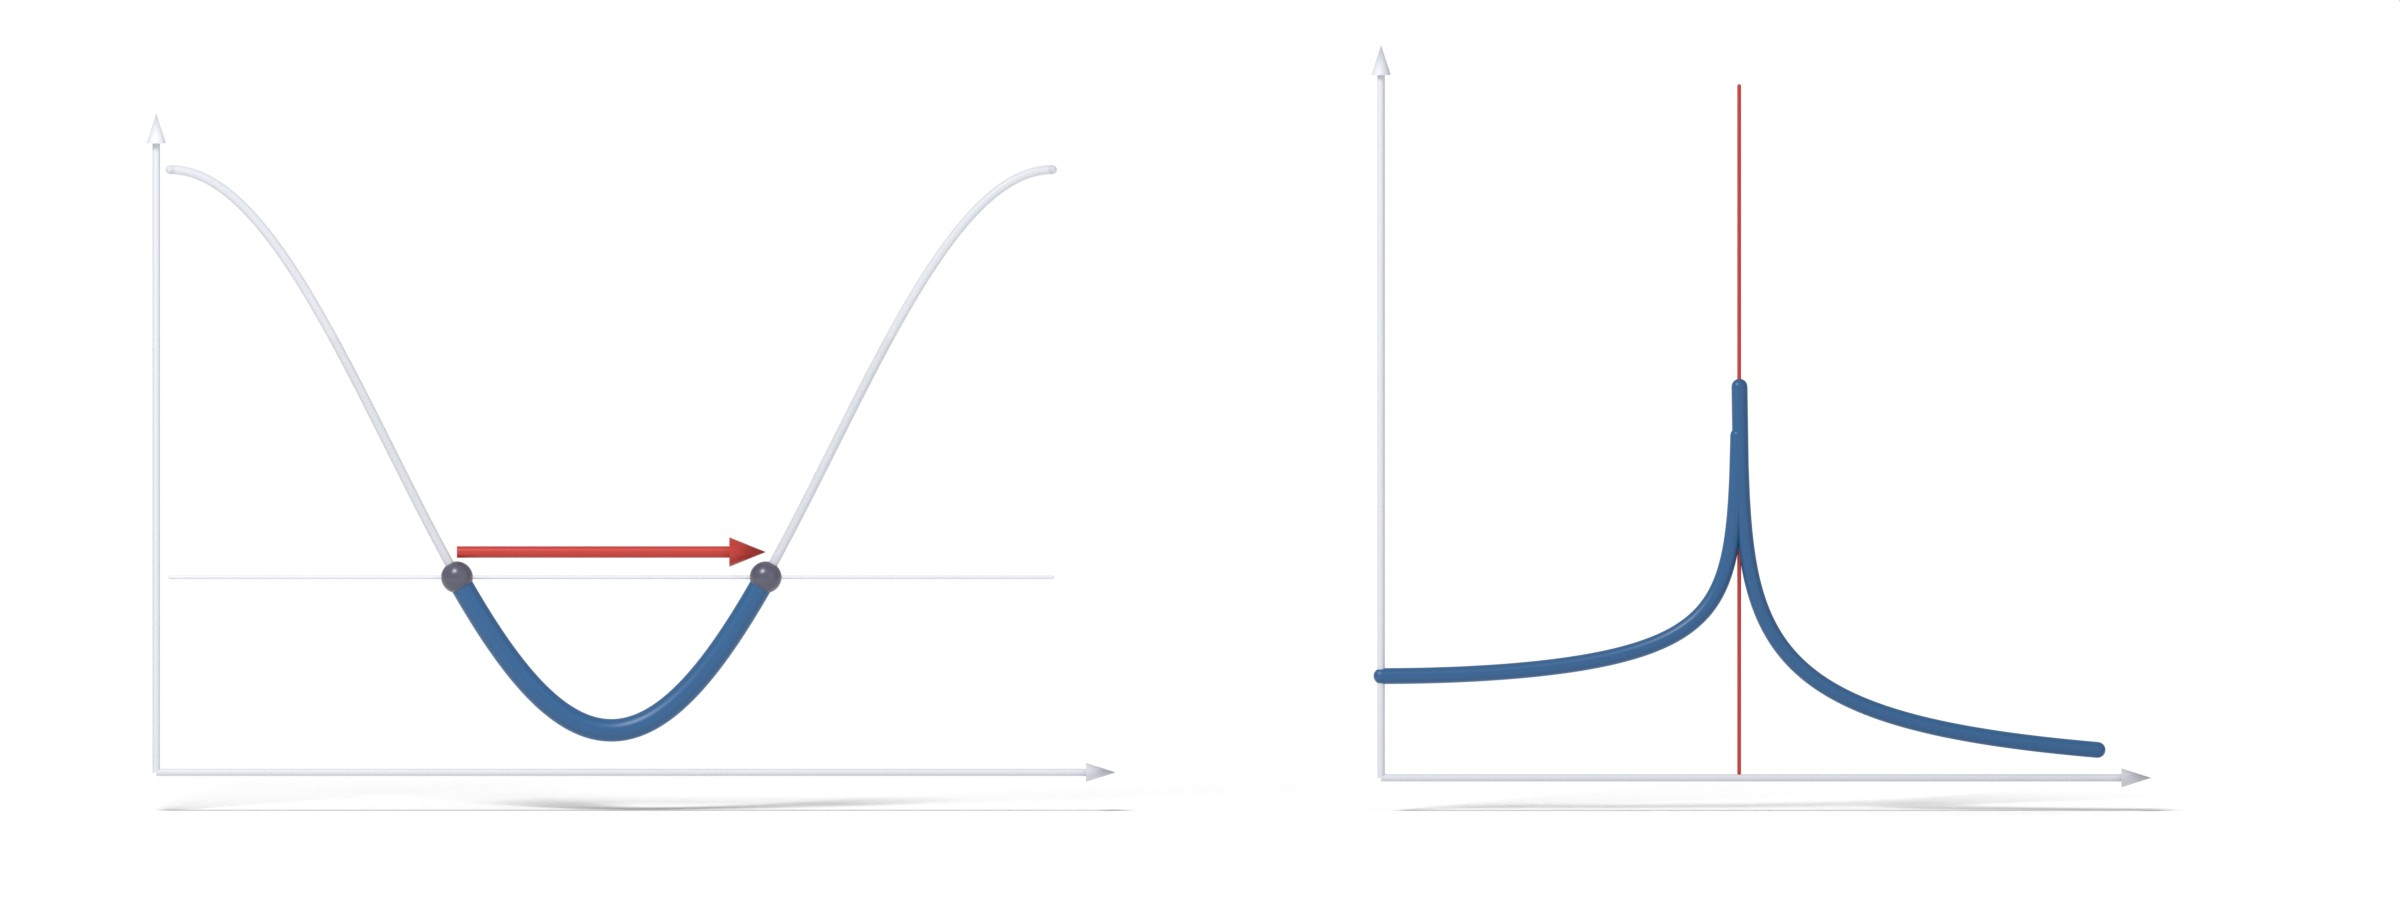
\includegraphics[width=\figw]{../blender/out/s09f01_nesting_ab.jpg}};
    % written by build_figure.sh; the painted part of the image
\path (0.0612\figw,0.0367\figw) rectangle (0.9075\figw,0.3558\figw);

    %% written by figlib.py; x and y in units of the image width
\coordinate (abak) at (0.4648\figw,0.0532\figw);
\coordinate (abaE) at (0.0651\figw,0.3277\figw);
\coordinate (abaq) at (0.2547\figw,0.1491\figw);
\coordinate (abakfm) at (0.1904\figw,0.0502\figw);
\coordinate (abakfp) at (0.3190\figw,0.0502\figw);
\coordinate (abaEF) at (0.4385\figw,0.1345\figw);
\coordinate (abapanel) at (0.0593\figw,0.3394\figw);
\coordinate (abbq) at (0.8962\figw,0.0509\figw);
\coordinate (abbchi) at (0.5755\figw,0.3561\figw);
\coordinate (abb2kf) at (0.7247\figw,0.0467\figw);
\coordinate (abbone) at (0.5755\figw,0.1357\figw);
\coordinate (abbpanel) at (0.5551\figw,0.3689\figw);

    \node[pnl, anchor=south west] at (abapanel) {(a)};
    \node[pnl, anchor=south west] at (abbpanel) {(b)};
    \node[lbl, anchor=north east] at (abak) {$k$};
    \node[lbl, anchor=west, xshift=0.25cm] at (abaE) {$\varepsilon(k)$};
    \node[lbl, anchor=south, text=aqmbroken] at (abaq) {$q^\star=2k_F$};
    \node[lbl, anchor=north] at (abakfm) {$-k_F$};
    \node[lbl, anchor=north] at (abakfp) {$k_F$};
    \node[lbl, anchor=south east, text=aqmmuted] at (abaEF) {$E_F$};
    \node[lbl, anchor=north east] at (abbq) {$q$};
    \node[lbl, anchor=west] at (abbchi) {$\chi_0(q)/D(E_F)$};
    \node[lbl, anchor=north, text=aqmbroken] at (abb2kf) {$2k_F$};
    \node[lbl, anchor=east] at (abbone) {$1$};
  \end{scope}
  \begin{scope}[shift={(10.70cm,0.00cm)}]
    \setlength{\figw}{4.90cm}
    \node[overlay, anchor=south west, inner sep=0pt] at (0,0)
      {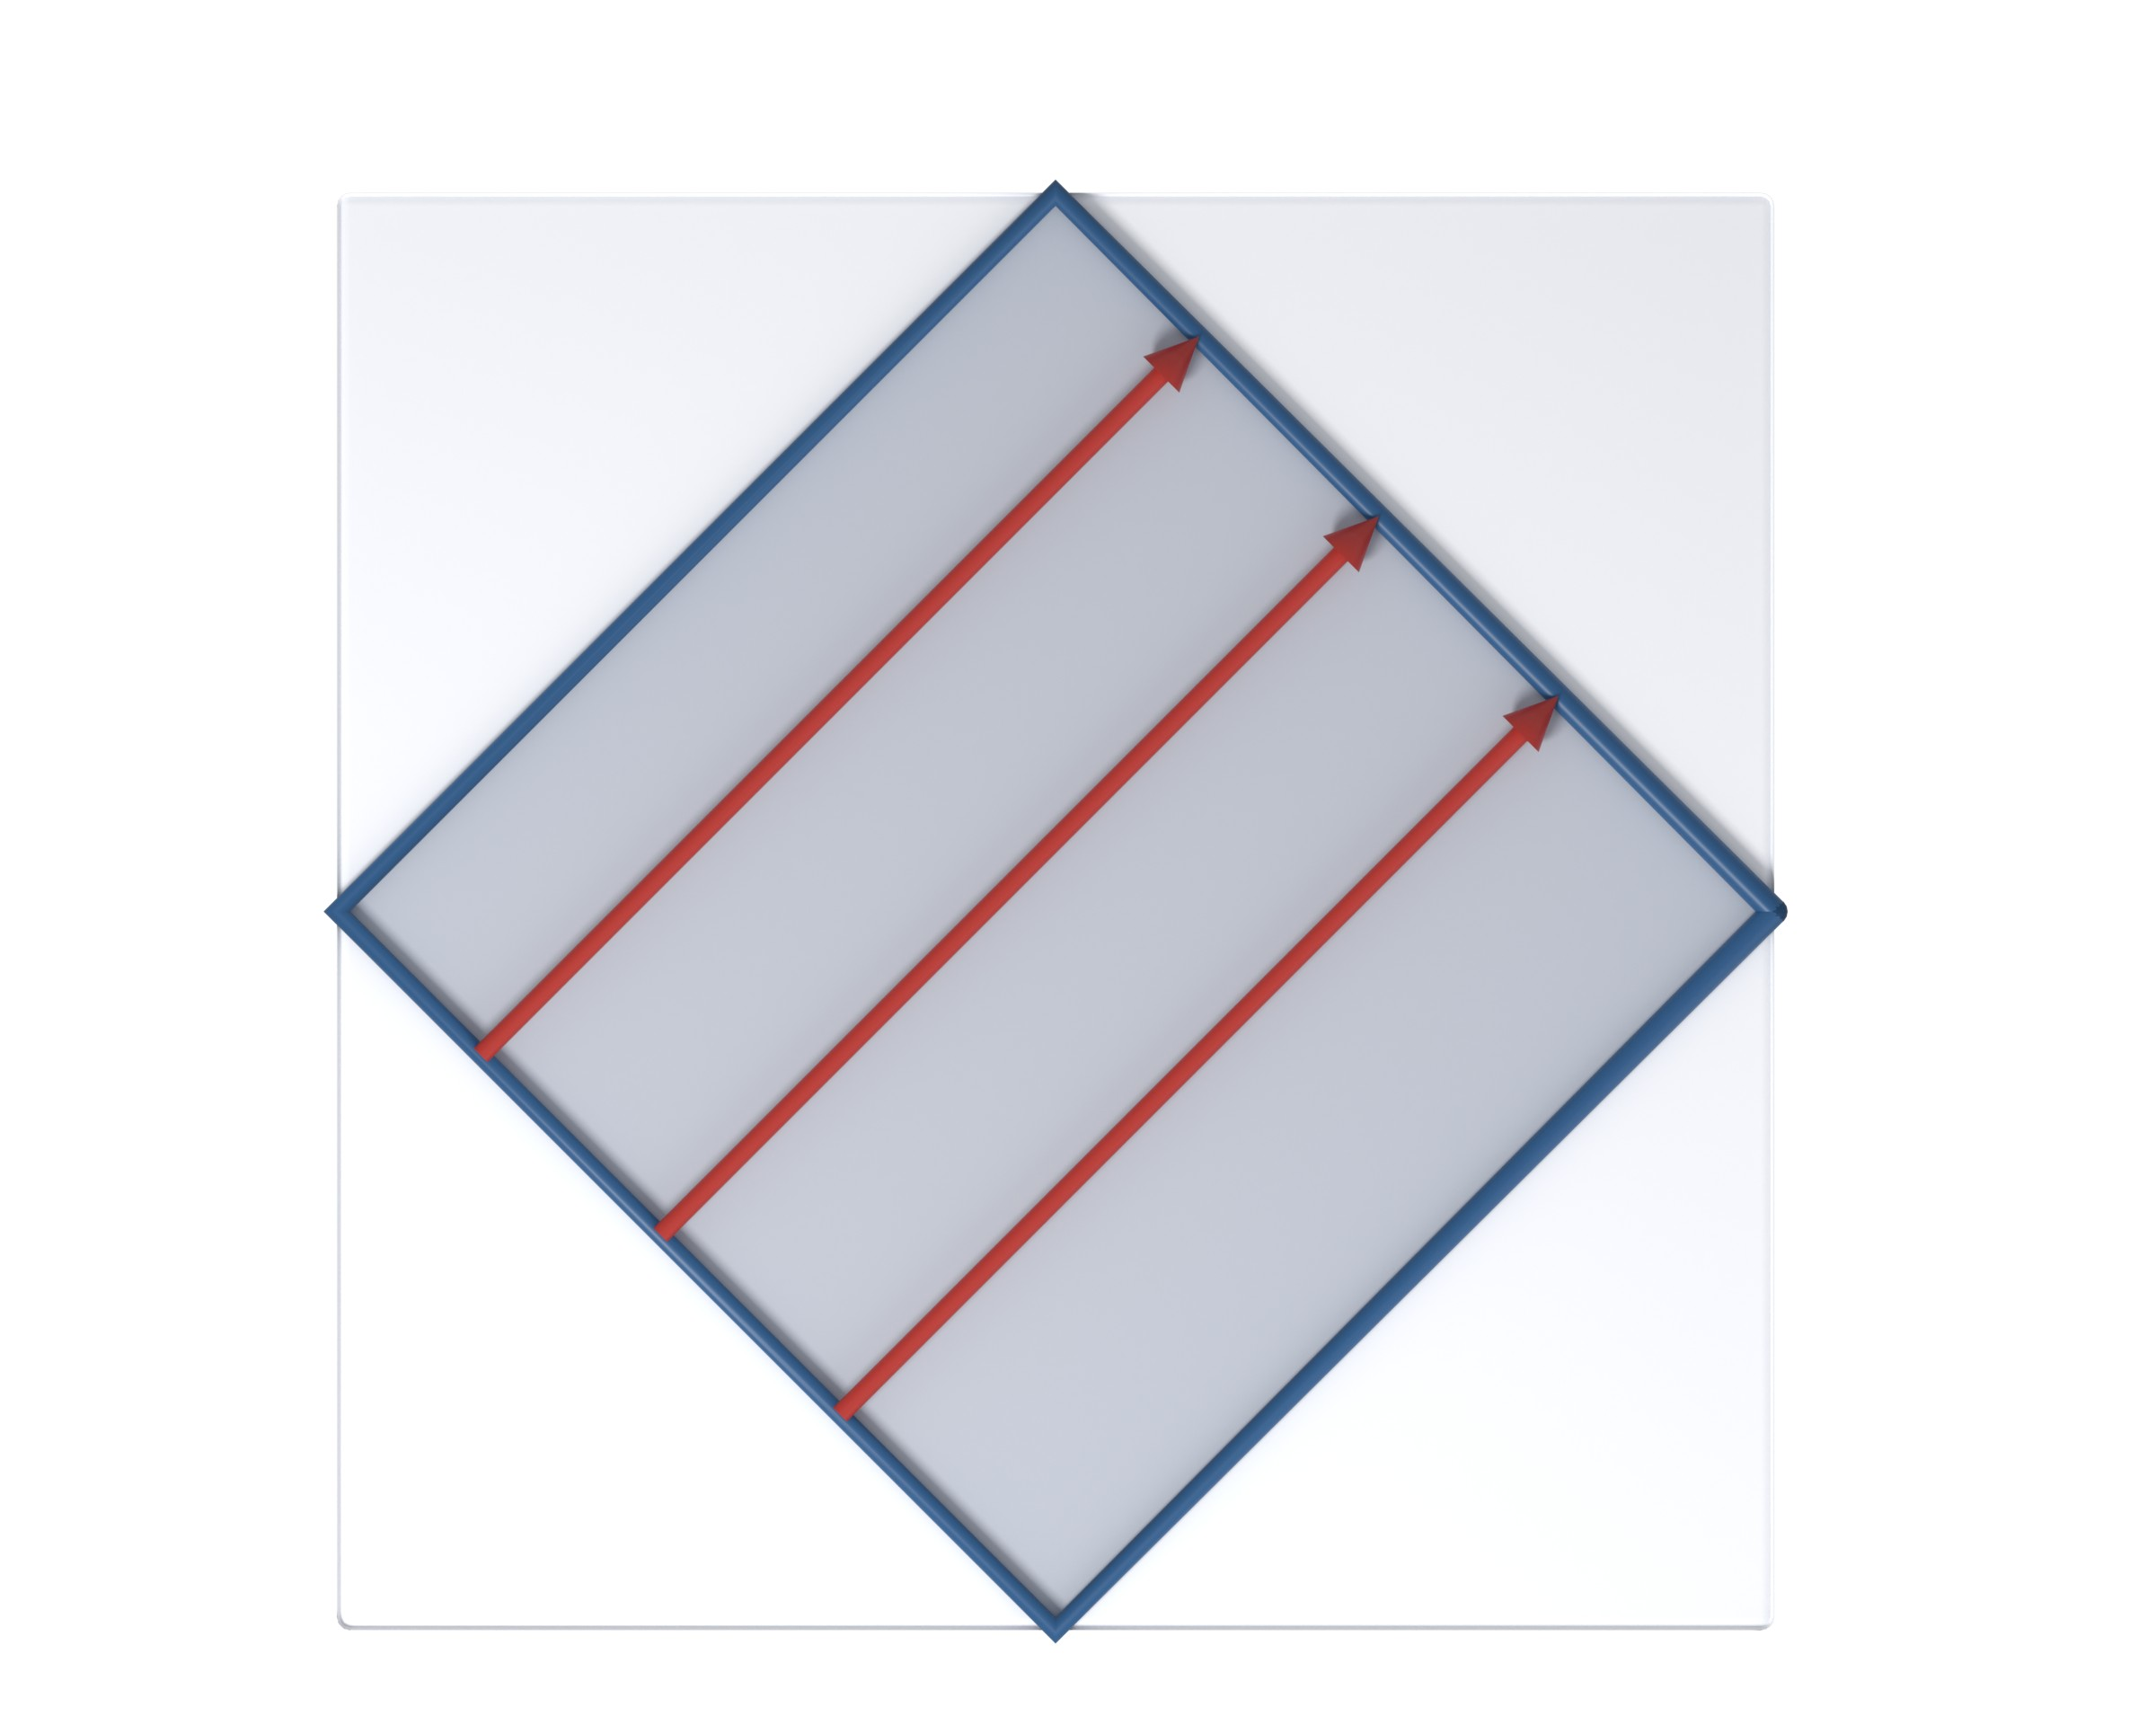
\includegraphics[width=\figw]{../blender/out/s09f01_nesting_c.jpg}};
    % written by build_figure.sh; the painted part of the image
\path (0.1500\figw,0.0333\figw) rectangle (0.8296\figw,0.7125\figw);

    %% written by figlib.py; x and y in units of the image width
\coordinate (ckO) at (0.4896\figw,0.3731\figw);
\coordinate (ckx) at (0.8958\figw,0.3731\figw);
\coordinate (cky) at (0.4896\figw,0.7793\figw);
\coordinate (cQ) at (0.1663\figw,0.0498\figw);
\coordinate (cpanel) at (0.1354\figw,0.7585\figw);

    \node[pnl, anchor=south west] at (cpanel) {(c)};
    \draw[axarrow] (ckO) -- (ckx);
    \draw[axarrow] (ckO) -- (cky);
    \node[axlbl, anchor=north] at (ckx) {$k_x$};
    \node[axlbl, anchor=west] at (cky) {$k_y$};
    \node[lbl, anchor=south west, text=aqmbroken, fill=white, fill opacity=0.85, text opacity=1, inner sep=0.8pt] at (cQ) {$Q=(\pi,\pi)$};
  \end{scope}
\end{tikzpicture}
\end{document}
